\includegraphics[height=1.25cm]{images/pictograms/benchmark}
\includegraphics[height=1.25cm]{images/pictograms/FEM}

%%%%%%%%%%%%%%%%%%%%%%%%%%%%%%%%%%%%%%%%%%%%%%%%%%%%%%%%%%%%%%%%%%%%%%%%%%%%%%%%%%%%%%%%%%%%%%%%%%%

%\lstinputlisting[language=bash,basicstyle=\small]{python_codes/fieldstone_18/keywords.key}

\begin{center}
\inpython
{\small Code: \url{https://github.com/cedrict/fieldstone/tree/master/python_codes/fieldstone_18}}
\end{center}

\par\noindent\rule{\textwidth}{0.4pt}

Last revision: Feb. 7th, 2025.

\par\noindent\rule{\textwidth}{0.4pt}

%%%%%%%%%%%%%%%%%%%%%%%%%%%%%%%%%%%%%%%%%%%%%%%%%%%%%%%%%%%%%%%%%%%%%%%%%%%%%%%%%%%%%%%%%%%%%%%%%%%

The code relies on \QtwoQone elements.
Each element has $m_V=9$ vertices so in total $ndof_V\times m_V=18$ velocity dofs and 
$ndof_P*m_P=4$ pressure dofs. The total number of 
velocity dofs is therefore $NfemV=NV \times ndofV$ while the total number of
pressure dofs is $NfemP=NP\times ndofP$. The total number of dofs is then $Nfem=NfemV+NfemP$.

As a consequence, matrix $\K$ has size $NfemV,NfemV$ and matrix $\G$ has size $NfemV,NfemP$.
Vector $f$ is of size $NfemV$ and vector $h$ is of size $NfemP$.  

When needed the pressure nullspace is removed 
by imposing (Lagrange multiplier) that $\int_\Omega p \; dV=0$.

The following figure shows the layout of velocity and pressure nodes
for a $4\times 3$ element mesh:
\begin{center}
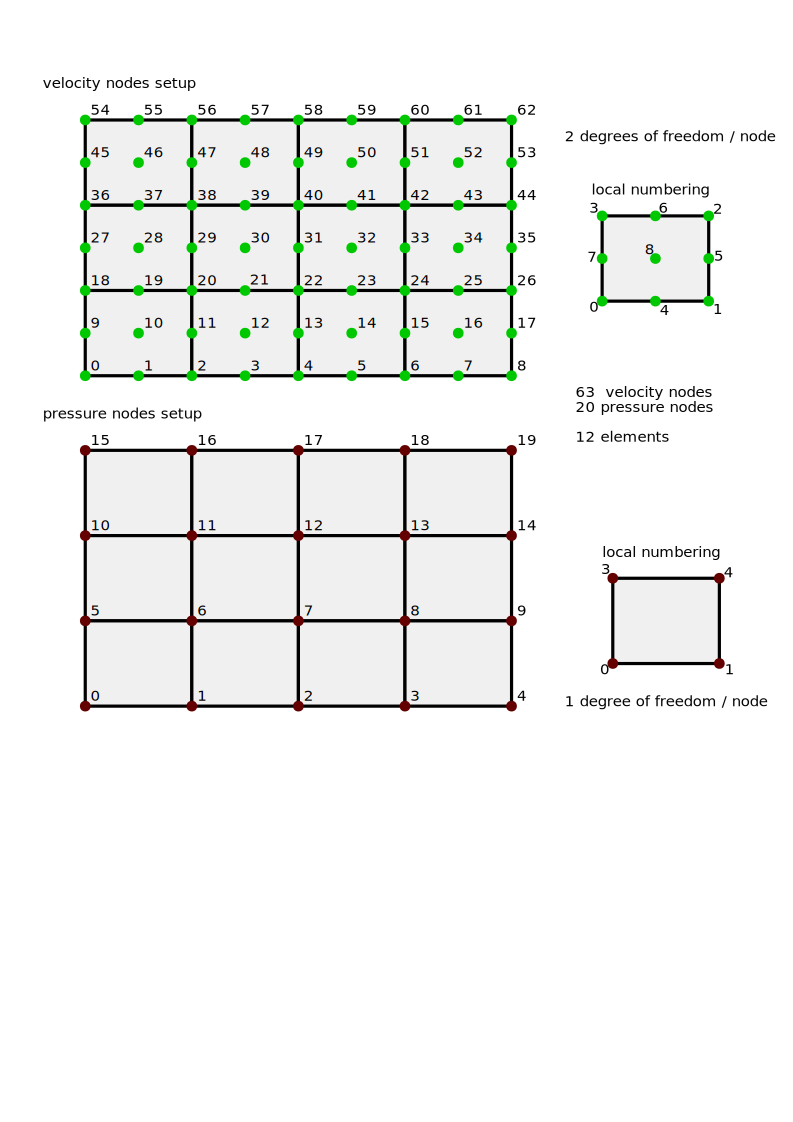
\includegraphics[width=10cm]{python_codes/fieldstone_18/images/q2q1setup}
\end{center}

%-----------------------------------------
\subsection*{Donea \& Huerta benchmark ({\tt bench=1})}
The details of the numerical setup are presented in Section \ref{MMM-mms1}.

\begin{center}
\includegraphics[width=7cm]{python_codes/fieldstone_18/results/mms/vel}
\includegraphics[width=7cm]{python_codes/fieldstone_18/results/mms/pressure}\\
{\captionfont Velocity and pressure fields for $32\times 32$ elements grid}
\end{center}

\begin{center}
\includegraphics[width=12cm]{python_codes/fieldstone_18/results/mms/errors}\\
{\captionfont Velocity and pressure error convergence for both nullspace removal 
techniques. The zero average pressure approach yields smaller errors.}
\end{center}

\newpage
%-----------------------------------------
\subsection*{Burman \& Hansbo manufactured solution ({\tt bench=4})}

The details of the numerical setup are presented in Section \ref{MMM-ss:mms_buha06}.
The velocity and pressure fields are given in the unit square by
\begin{eqnarray}
u(x,y) &=& 20xy^3 \nn\\
v(x,y) &=& 5x^4-5y^4 \nn\\
p(x,y) &=& 60x^2y -20y^3 -5
\end{eqnarray}
The analytical velocity is prescribed on all sides of the domain.

\begin{center}
\includegraphics[width=7cm]{python_codes/fieldstone_18/results/buha06/vel}
\includegraphics[width=7cm]{python_codes/fieldstone_18/results/buha06/p}\\
{\captionfont Velocity and pressure fields for $64\times 64$ elements grid}
\end{center}

\begin{center}
\includegraphics[width=8cm]{python_codes/fieldstone_18/results/buha06/errorsV}
\includegraphics[width=8cm]{python_codes/fieldstone_18/results/buha06/errorsP}\\
{\captionfont Velocity and pressure error convergence. Zero average.}
\end{center}

The conclusion is clear (and expected): there is no good reason 
to run such higher numbers of quadrature points.


\newpage
%----------------------------------------------------
\subsection*{Stokes sphere benchmark ({\tt bench=2})}

The setup is described in Section~\ref{MMM-ss:stokes_sphere2D}.
The domain is the unit square.
A sphere of radius 0.123456789 is placed in the middle of the domain. 
Its density is 1.01 while the density of the surrounding fluid is 1,
while its viscosity is 1000 times larger than the viscosity of the fluid.
Gravity is pointing downward with $|g|=1$.
There is no analytical solution to this problem.
Either no-slip or free-slip boundary conditions are prescribed on all 
sides.

\subsubsection*{Free-slip boundary conditions (FS)}

\begin{center}
\includegraphics[width=5.7cm]{python_codes/fieldstone_18/results/sphere/FS/vel}
\includegraphics[width=5.7cm]{python_codes/fieldstone_18/results/sphere/FS/press}
\includegraphics[width=5.7cm]{python_codes/fieldstone_18/results/sphere/FS/divv}\\
{\captionfont Velocity, pressure and velocity divergence fields for $48\times 48$ 
elements grid and $3^2$ quadrature points per element.}
\end{center}






\subsubsection*{No-slip boundary conditions (NS)}

\begin{center}
\includegraphics[width=5.7cm]{python_codes/fieldstone_18/results/sphere/NS/vel}
\includegraphics[width=5.7cm]{python_codes/fieldstone_18/results/sphere/NS/press}
\includegraphics[width=5.7cm]{python_codes/fieldstone_18/results/sphere/NS/divv}\\
{\captionfont Velocity, pressure and velocity divergence fields for $48\times 48$ 
elements grid and $3^2$ quadrature points per element.}
\end{center}




\newpage
%-----------------------------------------
\subsection*{Sinking block benchmark ({\tt bench=3})}

The setup is described in Section~\ref{MMM-ss:sinking_block} of part 1.
The domain is the unit square.
A block of density $\rho=1.01$ is placed in a fluid of density $\rho=1$.
The gravity is vertical and pointing downward with $|\vec{g}|=1$.
The function for $b_y$ is then:
\begin{lstlisting}
def by(x,y):
    [...]
    if abs(x-.5)<0.0625 and abs(y-0.5)<0.0625:
       val=-1.01
   else:
      val=-1.
\end{lstlisting}
The block is 1000 times more viscous than the fluid:
\begin{lstlisting}
def eta(x,y):
    [...]
    if bench==3:
       if abs(x-.5)<0.0625 and abs(y-0.5)<0.0625:
          val=1000
       else:
          val=1
\end{lstlisting}





\subsubsection*{Free slip boundary conditions (FS)}

\begin{center}
\includegraphics[width=7cm]{python_codes/fieldstone_18/results/block/FS/vel}
\includegraphics[width=7cm]{python_codes/fieldstone_18/results/block/FS/press}\\
{\captionfont Velocity and pressure fields for $48\times 48$ elements grid and $3^2$
quadrature points per element.}
\end{center}


\begin{center}
\includegraphics[width=5.7cm]{python_codes/fieldstone_18/results/block/vrms}
\includegraphics[width=5.7cm]{python_codes/fieldstone_18/results/block/max_vel}\\
\includegraphics[width=5.7cm]{python_codes/fieldstone_18/results/block/min_u}
\includegraphics[width=5.7cm]{python_codes/fieldstone_18/results/block/max_u}\\
\includegraphics[width=5.7cm]{python_codes/fieldstone_18/results/block/min_v}
\includegraphics[width=5.7cm]{python_codes/fieldstone_18/results/block/max_v}\\
\includegraphics[width=5.7cm]{python_codes/fieldstone_18/results/block/min_p}
\includegraphics[width=5.7cm]{python_codes/fieldstone_18/results/block/max_p}\\
\includegraphics[width=5.7cm]{python_codes/fieldstone_18/results/block/profile_u_FS}
\includegraphics[width=5.7cm]{python_codes/fieldstone_18/results/block/profile_v_FS}
\includegraphics[width=5.7cm]{python_codes/fieldstone_18/results/block/profile_p_FS}
\end{center}

%.....................................................
\subsubsection*{No slip boundary conditions (NS)}

\begin{center}
\includegraphics[width=5.7cm]{python_codes/fieldstone_18/results/block/NS/u}
\includegraphics[width=5.7cm]{python_codes/fieldstone_18/results/block/NS/v}
\includegraphics[width=5.7cm]{python_codes/fieldstone_18/results/block/NS/p}\\
{\captionfont Velocity and pressure fields for $32\times 32$ elements grid and $3^2$
quadrature points per element.}
\end{center}

Velocity and pressure are also measured on a vertical line going through
the middle of the domain/block (the lithostatic pressure is 
subtracted from the computed full pressure so that what is plotted is the 
dynamic pressure):
\begin{center}
\includegraphics[width=5.7cm]{python_codes/fieldstone_18/results/block/profile_u_NS}
\includegraphics[width=5.7cm]{python_codes/fieldstone_18/results/block/profile_v_NS}
\includegraphics[width=5.7cm]{python_codes/fieldstone_18/results/block/profile_p_NS}
\end{center}
As expected, the $x$ component of the velocity is zero because of symmetry.


\newpage
%----------------------------------------------------
\subsection*{Inclusion in pure shear ({\tt bench=5})}

(this setup was created for Philippe Yamato of Rennes University)

The inclusion is placed at the origin and has a radius 0.1, while the domain is the 
unit square. Viscosity inside the inclusion is 1 while the matrix viscosity is 1000.
Free slip is prescribed on the left and bottom boundary while 
$u=-1$ is prescribed on the right boundary and $v=+1$ on the top.

\begin{center}
\includegraphics[width=5.7cm]{python_codes/fieldstone_18/results/inclusion/eta}
\includegraphics[width=5.7cm]{python_codes/fieldstone_18/results/inclusion/vel}
\includegraphics[width=5.7cm]{python_codes/fieldstone_18/results/inclusion/press}\\
{\captionfont Resolution $256\times 256$.}
\end{center}

Note that viscosity is prescribed on quadrature levels, which in this case 
is likely to generate large errors/jumps around the inclusion surface.

\begin{verbatim}
For 256x256 mesh on my laptop:
setup: grid points: 0.128 s
setup: connectivity: 0.242 s
setup: boundary conditions: 0.151 s
build FE matrix: 284.284 s
assemble blocks: 0.003 s
solve time: 804.607 s
\end{verbatim}



